
\section{Results: Part I}

In order to get a representation of the mechanism we run 300 randomly initiated scenarios, with the experimental design capable of accepting more data at a later point. We then extract the lifetimes from the diagonal of the jacobian, and convert them into vectors representing the duration of all 3 days for each simulation. These vectors are then compared against eachother to find species of similar lifetimes, which follow a like response to the diurnal cycle. This is done through the use of euclidian and cosine similarities. 

\subsection{Temporal Lifetime Vector Comparison}
First we wish to explore the results of a single simulation. This will help establish the thresholds and methodology that is to be used in future examples. As we do not wish to lump inorganics, we remove these from the program and generate all the pairwise interactions between species. We compute the euclidean and cosine distances for all remaining reaction pairs (88410 pairs) across the entirety of the single calculation. These are then plotted on separate axis, and coloured using the geometric mean, \autoref{fig:metric}. \\

Since there are $n^2$ different combinations, this process can be lengthy to compute. Moreover the number of nodes present makes it difficult to visually determine which couplets to lump together, especially when they are overlaying eachother, as in \autoref{fig:morig}. To overcome this we apply a force graph simulation to each node. Here a strong force pulls them towards their true location, whist a collision/repulsive force ensures that there exists no overlap between nodes. Although some information loss may be incurred this way, it does enable us to interactively determine which pairs belong to which points.   

Plotting the data this way provides an approximate view of how lifetimes change within the system. \autoref{fig:density2} shows the distribution of values across both metrics. Here we see that although there is some difference the cosine difference can be used as an indicator for exploring further. This is useful since the cosine difference is a matrix operation and can produce near instant results in the form of the output relationship matrix. The euclidean distance however must be computed for each coupling individually as it requires taking the difference between the temporal lifetime arrays of each species. This means that rather than computing the euclidean distance for all permutaions of species, we can compute only those whose cosine distances suggest potentially promising results.  



\begin{figure}[H]
\begin{subfigure}{.5\textwidth}
  \centering
  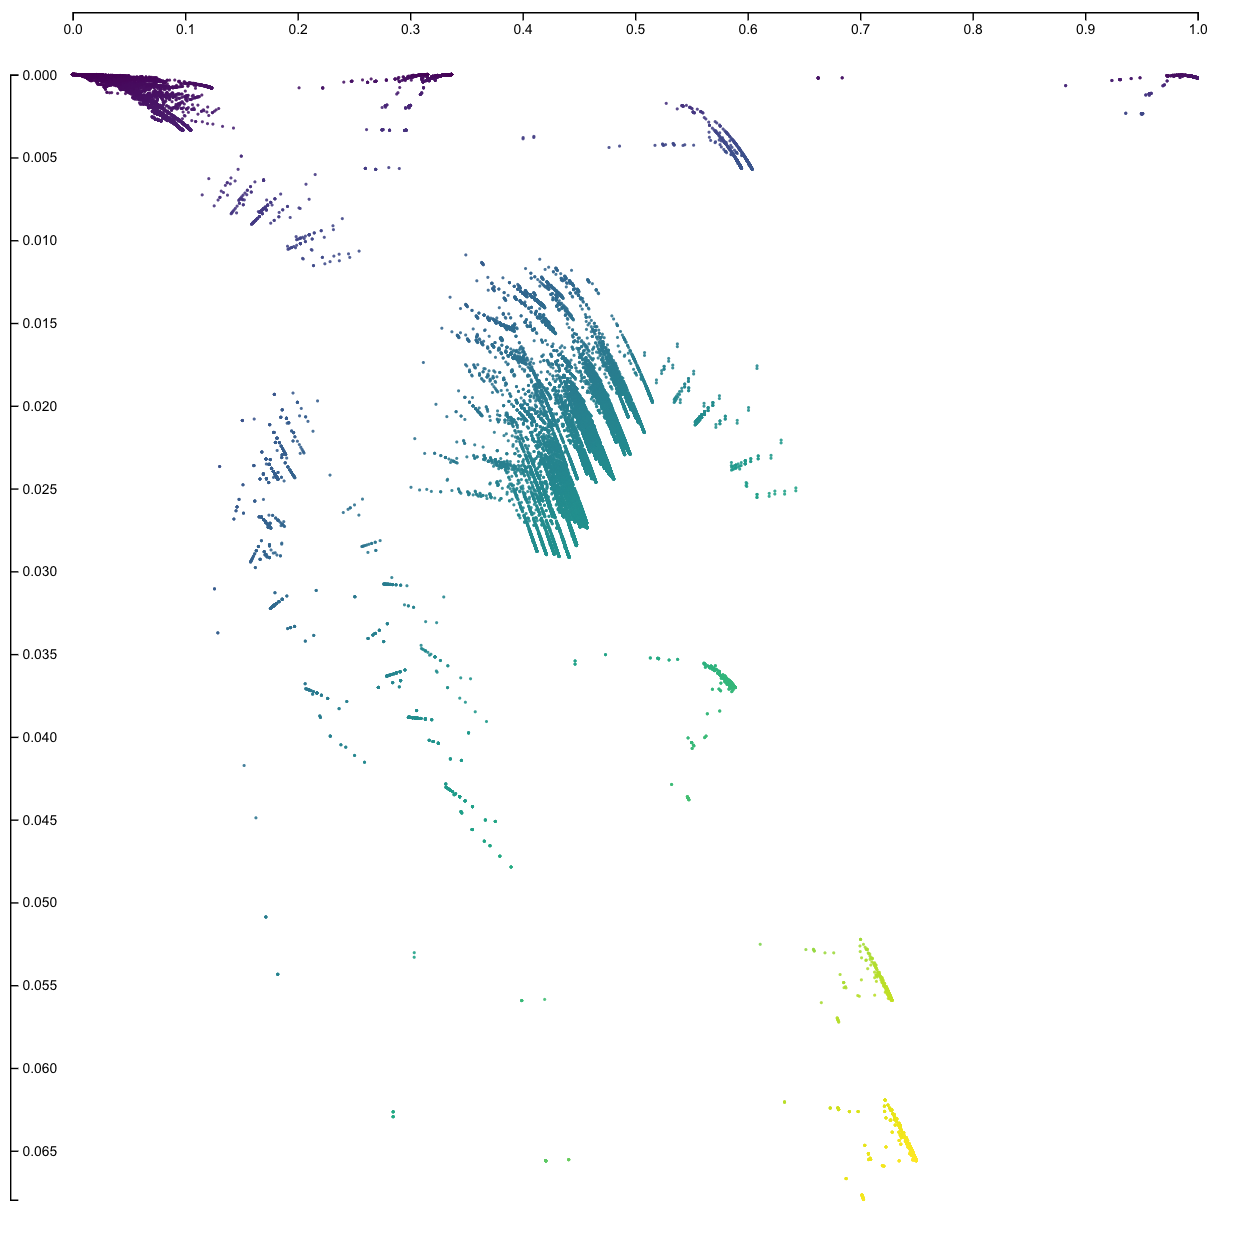
\includegraphics[width=\textwidth]{fig/metric-1.png}
  \label{fig:morig}
  \caption{Original}
\end{subfigure}%
\begin{subfigure}{.5\textwidth}
  \centering
  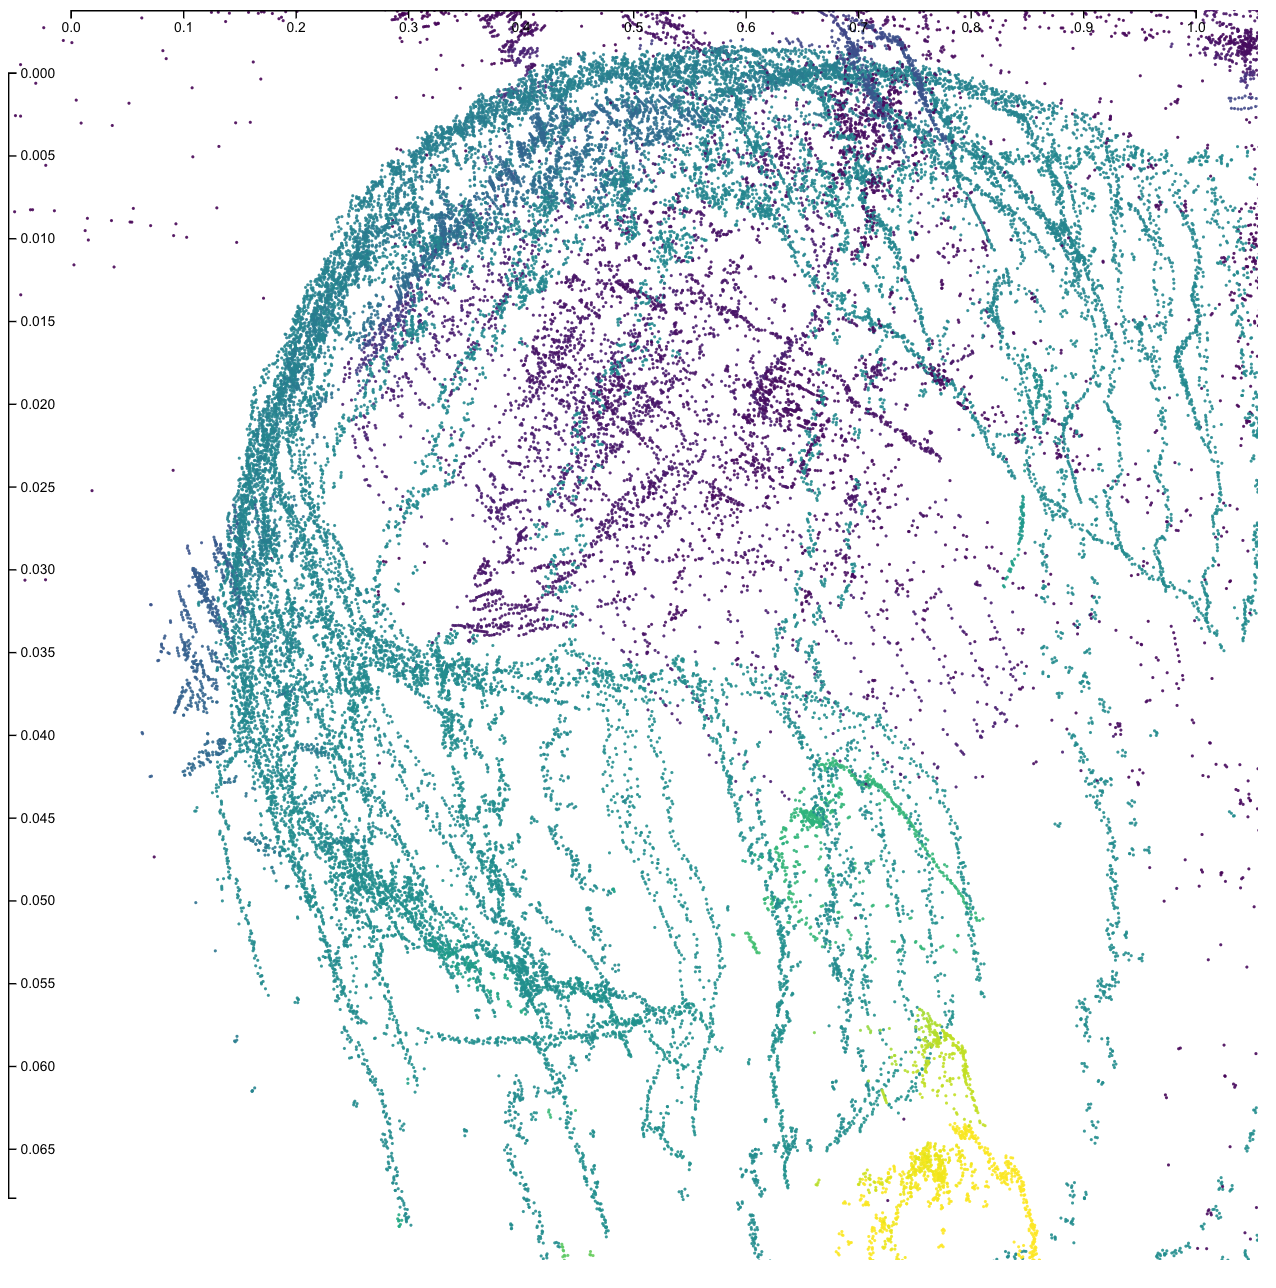
\includegraphics[width=\textwidth]{fig/metric0.png}
  \label{fig:m1}
  \caption{First collision detection timestep, before attractive forces have fully kicked in.}
\end{subfigure}

\caption{Showing the evolution from the original overlaid locations, \autoref{fig:morig} to the slightly more accessible (interactively) \autoref{fig:metric}}
\end{figure}


\begin{figure}

\begin{subfigure}{.5\textwidth}
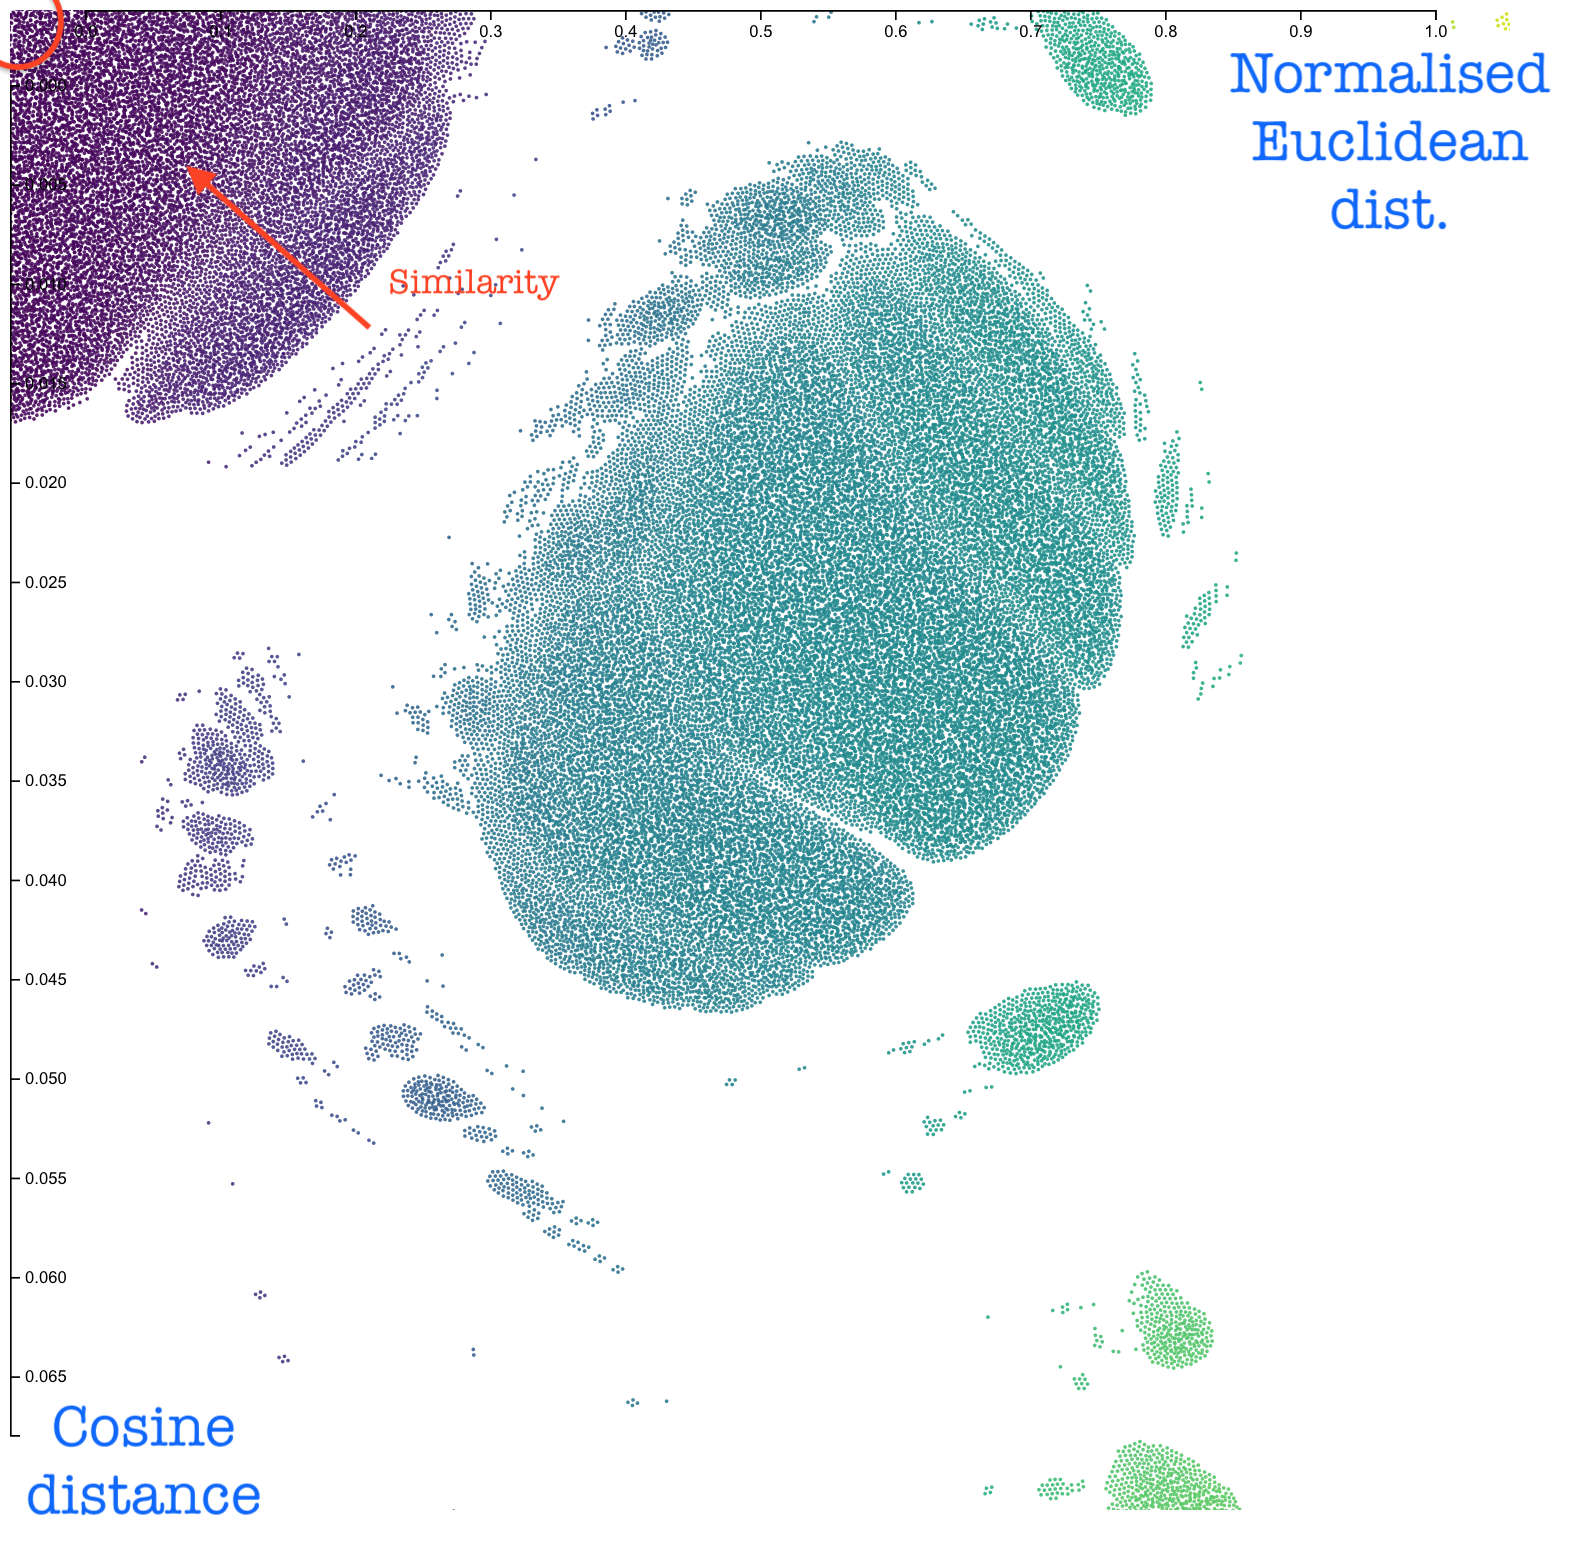
\includegraphics[width=\textwidth]{fig/metric.png}
\label{fig:metric}
\caption{Interactive, non overlapping plot of normalised euclidian distance across the x axis against the cosine distance on the y. The colouring is the geometric mean between them.}
\end{subfigure}
\begin{subfigure}{.5\textwidth}
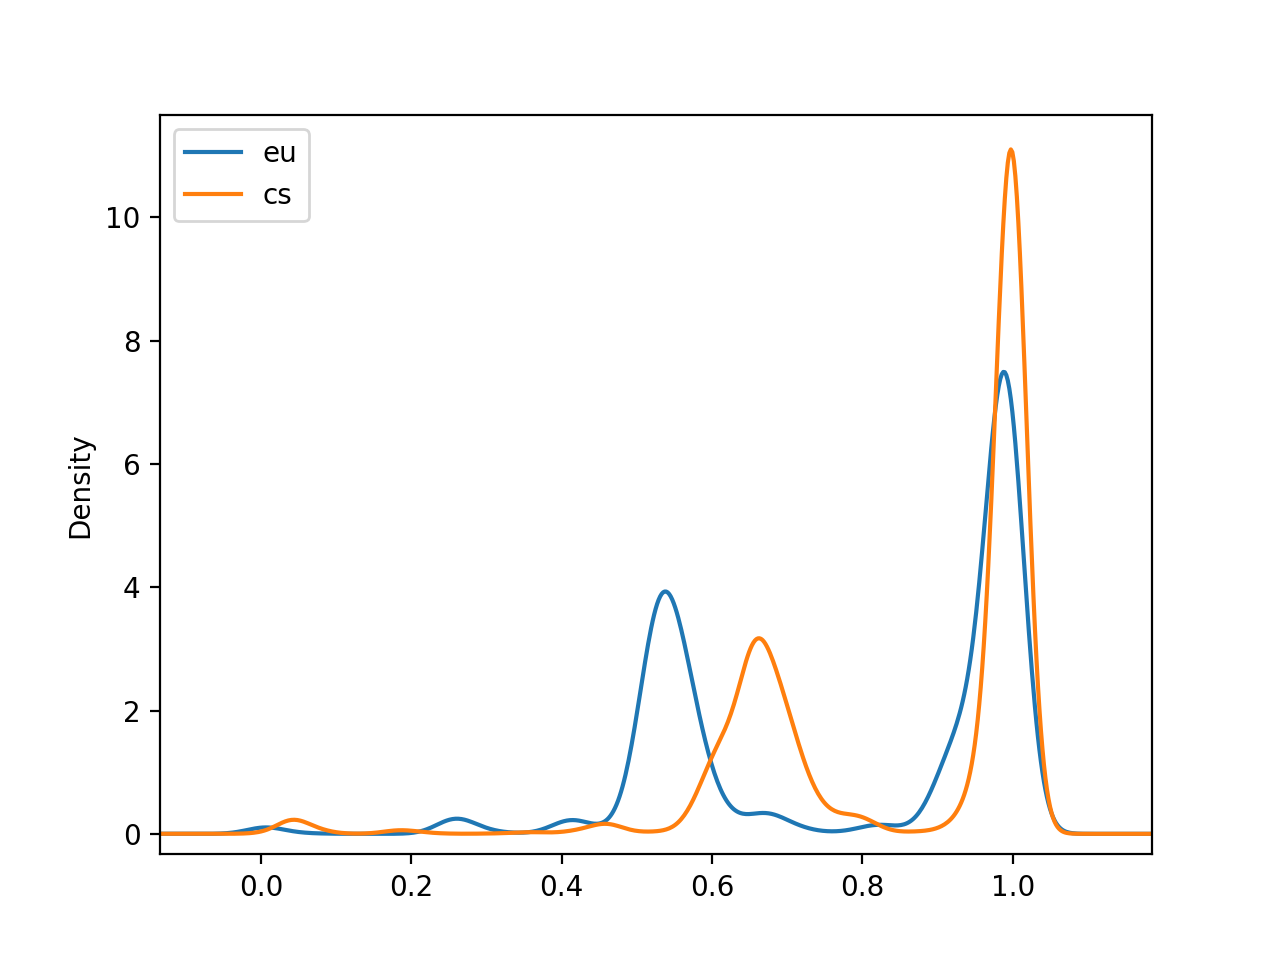
\includegraphics[width=\textwidth]{fig/metric_density.png}
\label{fig:density2}
\caption{Gaussian Kernel Density Estimate plot showing the distributions present for each distance metric}
\end{subfigure}
\caption{Showing the evolution from the original overlaid locations, \autoref{fig:morig} to the slightly more accessible (interactively) \autoref{fig:metric}}
\end{figure}


\subsection{Viewing the similarity graph}

One method to simplify this is to convert to the pairwise interaction list into a fully connected graph. Here we have individual species, pulled together by the similarity (geometric mean) between each two nodes.
Unfortunately in being a complete graph of  421 species and 88410 links, this is quite difficult to visualise without forming a \emph{hairball} [fig a]. As a means of filtering the results we trim the weakest links in sequence. This produces rings of densely connected species based on lifetime thresholds which corresponds to the different types of chemsitry species undergo \\


